\documentclass[reprint,amsmath,amssymb,aps,pra,floatfix]{revtex4-2}


\usepackage{graphicx}% Include figure files
\usepackage[caption=false]{subfig}
\usepackage{dcolumn}% Align table columns on decimal point
\usepackage{bm}% bold math
%\usepackage{hyperref}% add hypertext capabilities
\usepackage[mathlines]{lineno}% Enable numbering of text and display math
\usepackage{mathtools}
\usepackage{physics}
\usepackage{times,txfonts}
\usepackage{hyperref}
% \linenumbers\relax % Commence numbering lines



%\usepackage[showframe,%Uncomment any one of the following lines to test
%%scale=0.7, marginratio={1:1, 2:3}, ignoreall,% default settings
%%text={7in,10in},centering,
%%margin=1.5in,
%%total={6.5in,8.75in}, top=1.2in, left=0.9in, includefoot,
%%height=10in,a5paper,hmargin={3cm,0.8in},
%]{geometry}

% \newcommand{\bra}[1]{\langle #1 |}
% \newcommand{\ket}[1]{| #1 \rangle}
% \newcommand{\braket}[2]{\langle #1| #2\rangle}
% \newcommand{\pdv}[2]{\frac{\partial #1}{\partial #2}}
% \newcommand{\Tr}{\text{Tr}}
\renewcommand{\var}[1]{\text{var} (#1) }
\newcommand{\cov}[2]{\text{cov} (#1, #2) }
\DeclarePairedDelimiter\floor{\lfloor}{\rfloor}

\begin{document}

\preprint{APS/123-QED}

\title{Quantum precison bounds for passive surface metrology}% Force line breaks with \\

\author{Jernej Frank}
\email{jernej.frank@physics.ox.ac.uk}
\affiliation{%
 Department of Physics, University of Oxford, Oxford, OX1 3PU, UK
}

\author{Tommaso Tufarelli}
\email{who wants to be corresponding?}
\author{Gerardo Adesso}
\affiliation{%
 School of Mathematical Sciences, University of Nottingham, University Park, Nottingham NG7 2RD, United Kingdom
}%
\author{Samanta Piano}
\affiliation{%
 Manufacturing Metrology Team, Faculty of Engineering, University of Nottingham, Nottingham NG7 2RD, United Kingdom
}%

\date{\today}% It is always \today, today,
             %  but any date may be explicitly specified

% With abstracts, I typically aim for a 5-sentence model that mirrors the structure of the rest of the paper:
% S1: what we know
% S2: what we don't
% S3: how you answer that question
% S4: what you find
% S5: why it's important
\begin{abstract}
We develop a general quantum-mechanical framework for the sub-wavelength localization of $N$ point sources, applicable to a variety of problems in passive surface metrology.
%Optical surface metrology comprises many techniques for estimating surface parameters. It offers a faster alternative over mechanical profilometry, with decreased accuracy due to the diffraction nature of optics and reliance on mathematical reconstruction models instead of measuring the surface directly.
%Our investigation into the precision bounds of optical methods has led us to propose novel measuring schemes that have the potential to revolutionise accuracy in optical surface metrology. By generalising the analysis of quantum and classical Fisher information from two-point source problems to an arbitrary number of point sources, we propose a discrete imaging model for its real-world continuous counterpart.
%We find that passive measurement schemes can improve accuracy in estimating descriptive parameters for surface defects. Our analysis opens the possibility that estimation parameters have a corresponding measurement basis vector that contributes most of the information necessary to estimate it. Lastly, the insights lead to improved measurement schemes in optical metrology and pave the way towards a general imaging description using parameter estimation approaches.
\end{abstract}



\maketitle

%\tableofcontents
\section{\label{sec:intro} Introduction}
Optical surface metrology analyses three-dimensional (3D) surfaces via non-contact probing using light \cite{leach2020advances,catalucci2022optical}. It captures a broader sample surface area faster than its contact counterparts, where a mechanical scan is needed. Since we have control over the illumination of the object, it is usually an active measurement and makes use of the apriori knowledge of the illumination for improved reconstruction  \cite{hocken2005optical}. However, due to the nature of light propagation, optical surface metrology is limited in its accuracy by the diffraction limit. In addition, due to its dependence on the object's properties (for example, reflectivity in metal) and surface estimation arising from underlying mathematical models instead of deriving it from the surface itself, the researchers use optical metrology cautiously \cite{mathia2011recent}.

Choosing the appropriate probe state in the illumination path classifies the techniques into three general reconstruction approaches \cite{marrugo2020state}: triangulation, time-of-flight (ToF), and wave interference. The measurement is split into multiple partial measurements (different illumination patterns, scanning along the z-axis, ...) or a single-shot measurement with heavy computational post-processing to extract the necessary information \cite{yang2022single, van2019deep, wang2021single, li2016single}. Combining different techniques into a single machine that allows the user to measure over a broader range while benefiting from a high-resolution measurement is popular.

We analyse optical surface metrology from the perspective of parameter estimation theory to derive ultimate precision bounds. It has been an actively developing field since the original analysis of estimating the distance between two-point sources that suggested a possibility of overcoming the classical diffraction limit\cite{tsang2016quantum}. Our approach builds on the previous results\cite{fiderer2021general,napoli2019towards, genoni2019non}, generalises the analysis to an arbitrary number of point sources in three dimensions, and proposes a discretisation model for its real object continuous counterpart.

We demonstrate our technique on the example of estimating the depth and width of a surface crack. To be as agnostic as possible, we limit ourselves to only passive measurement schemes in the image plane with no prior assumption on the illumination path. This allows us to include measurement examples on terrain where controlling the illumination path is impossible. While our approach is general for an arbitrary number of point sources, we showcase it on the toy model of three-point sources to relay the principles without getting lost in details. However, even with such a simplified model, we gain insights that help us propose possible measurement schemes worth investigating to improve accuracy using optical techniques.


\section{\label{sec:prelim} Preliminaries}
We summarise the terminology of parameter estimation theory and recap the non-orthogonal basis approach used to obtain the covariance matrix that encodes precision boundaries for the parameters in question.

\subsection{Parameter estimation theory}
We consider $m$ distinct parameters $\theta = (\theta_1,\theta_2,\dots,\theta_m)$ for which we aim to build estimators $ \hat{\theta} = (\hat{\theta}_1,\hat{\theta}_2,\dots,\hat{\theta}_m)$. For any estimation strategy, the error covariance matrix $\Sigma(\theta)$ is lower bounded by the classical Cramer-Rao bound \cite{helstrom1969quantum,braunstein1994statistical}, which in turn is lower bounded by the quantum Cramer-Rao bound \cite{lehmann2006theory,van2004detection}
\begin{align}
    \Sigma(\theta) \geq \frac{1}{N} J^{-1} \geq \frac{1}{N} H^{-1},
\end{align}
with $N$ being the number of measurements, $J$ the Fisher information matrix (FIM) and $H$ the quantum Fisher information matrix (QFIM). The inequalities are to be understood in the sense that $\Sigma(\theta) - \frac{1}{N} J^{-1}$  and $\Sigma(\theta) - \frac{1}{N} H^{-1}$ are positive semidefinite matrices.
If we implicitly define the symmetric logarithmic derivative (SLD) related to parameter $\theta_a$ ($a=1,2,\dots,m$) as
\begin{align}
   2\frac{\partial \rho}{\partial \theta_a} = \rho L_a+ L_a \rho,
\label{def:sld}
\end{align}
for a parameter-dependent density operator $\rho=\rho(\theta)$, we can express the QFIM as
\begin{align}
    H_{a,b} = \text{Tr} \left [ L_{a} \frac{\partial \rho}{\partial \theta_{b}} \right ].
\label{def:QFIM}
\end{align}
Similarly,  the FIM is defined as
\begin{align}
    J_{a,b} &= \int \ dr \ P(r|\theta) \frac{\partial}{\partial \theta_a}\left[ \ln P(r|\theta)\right] \frac{\partial}{\partial \theta_b}\left[ \ln P(r|\theta)\right]\\
            &= \int \ dr \ \frac{1}{P(r|\theta)} \frac{\partial P(r|\theta)}{\partial \theta_a}\frac{\partial P(r|\theta)}{\partial \theta_b},
\label{def:FIM}
\end{align}
with $P(r|\theta)$ the parameter-dependent probability distribution.

Since we are exploring classical measurements, it is reasonable to assume some photon loss, and the above definition will need a slight adjustment. The approach is based on Tsang's semi-classical treatment \cite{tsang2018subdiffraction}, assuming a Poissonian distribution
$    P(m|\theta) = \prod_j \frac{[\tau p_j(\theta)]^{n_j}}{n_j!} e^{-\tau p_j(\theta)}$,
with
\begin{align}
    p_j(\theta) &= \int dr \abs{\int dr' \phi_j^*(r') \psi(r-r')}^2 F(r|\theta) \nonumber \\
    &= \int dr \abs{ \braket{\phi_j}{\psi} }^2 F(r|\theta)
\label{eq:ms_prob}
\end{align}
being the mean power measured in a particular mode channel $\phi_j$ for an object $F(r|\theta)$ and    $\tau = \frac{\eta T}{\hbar \omega}$
the Poissonian rate expressed through  the detection efficiency $\eta$, the integration time $T$, and the  photon energy $\hbar \omega$. With this  modification, the classical FIM takes on a similar form
\begin{align}
    J_{a,b} = \tau \sum_j\frac{1}{p_j(\theta)} \pdv{p_j(\theta)}{\theta_a}  \pdv{p_j(\theta)}{\theta_b}.
\label{eq:FI_MS}
\end{align}
However, the advantage is that we do not need to measure all the photons. This becomes an important caveat that allows us to measure in multiple channels that do not necessarily need to be independent of each other.

\subsection{Non-orthogonal basis approach}
We will use a non-orthogonal basis to calculate the QFIM \cite{genoni2019non,napoli2019towards,fiderer2021general}. Given a generic basis $\{\ket{\psi_v}\}, v = 1,2,\dots,N$, which spans the subspace relevant to the estimation problem, we consider the Grammian matrix $G_{u,v}=\braket{\psi_u}{\psi_v}$. We can then expand all operators of interest as
\begin{align}
    \rho &= \sum_{u,v} R^{u,v} \ket{\psi_u}\bra{\psi_v} \\
    \pdv{\rho}{\theta_a} &= \sum_{u,v} D_a^{u,v} \ket{\psi_u}\bra{\psi_v}\\
    L_a &=  \sum_{u,v} L_a^{u,v} \ket{\psi_u}\bra{\psi_v},
\end{align}
which implicitly define the matrices ${R}, D_a$ and $L_a$. The key algebraic rule to keep in mind is that every index contraction must be accompanied by an instance of the Grammian matrix ${G}$. So, for example, the Lyapunov equation (\ref{def:sld}) for the $a-$th SLD becomes
\begin{align}
    2 {D}_a = {L}_a{G}{R} + {R}{G}{L}_a,
    \label{eq:sld_nonorthogonal}
\end{align}
while we can evaluate the QFIM elements as
\begin{align}
    H_{a,b} = \Re \Tr( R L_a  G L_b G).
    \label{eq:qfi_nonorthogonal}
\end{align}
If we are interested in estimating a different set of parameters, say $\Tilde{\theta}$, which can be expressed as functions of the original parameters $\theta$, then the corresponding QFIM is transformed by means of the Jacobian of the re-parametrization \cite{paris2009quantum},
\begin{align}
    \Tilde{H} = B H B^\top, \quad
    B_{\alpha,\beta} = \pdv{\theta_\beta}{\Tilde{\theta}_\alpha}.
    \label{def:jacobian}
\end{align}


\section{\label{sec:CR-bounds} Precision Bounds for discrete imaging models}
We wish to keep the analysis as general as possible, so we do not assume any {\it a priori} knowledge of the illumination. With this in mind, let us model the surface as a discrete grid of points in 3D space. Each point represents an emitter of photons that get collected by a lens. Assuming monocromatic light of wavelength $\lambda$ and a circular shape of the lens (the most common encounter), the photon's spatial probability profile in the image plane of a single point source is known as the point spread function of the imaging system and is described by a Gaussian beam:
%\begin{widetext}
\begin{equation}
\begin{aligned}
\label{def:psf}
    &\psi_v (x+\delta x_v,y+\delta y_v,z+\delta z_v) = \sqrt{\frac{1}{\pi}} \frac{i}{z+\delta z_v + i} \\
    &\times \exp{\frac{-i((x+\delta x_v)^2 + (y+ \delta y_v)^2)}{2(z+\delta z_v + i)} - ikz_R(z+\delta z_v)},
\end{aligned}
\end{equation}
%\end{widetext}
where $(x,y,z)$ are coordinates in the object plane, $(\delta x_v,\delta y_v,\delta z_v)$ are displacements of the point source $v$ from the origin in the object plane, $k= 2\pi / \lambda$ is the wave vector, and $z_R$ the Rayleigh length. We re-normalised the coordinate system to use the relative length scales $x \rightarrow \sqrt{k/z_R}x$ and $ z \rightarrow z/z_R$.

We can then represent the object's complete distribution as a superposition of $N$ point sources
\begin{align}
    \psi = \sum_v^N I_v \psi_v (x+\delta x_v, y+\delta y_v,z+\delta z_v),
\end{align}
with $I_v$ the relative intensity and (assuming no photon loss) $\sum_v I_v = 1$.

\subsection{\label{subsec:QFI_incoherent} Quantum Cramer-Rao bound for incoherent point sources}
We can represent an object consisting of incoherent point sources by the following density matrix:
\begin{align}
    R = \sum_v^N I_v \ket{\psi_v}\bra{\psi_v}
\end{align}
where each point source is displaced from the origin,
\begin{align}
    \ket{\psi_v} = \int \psi_v (x+\delta x_v,y+\delta y_v,z+\delta z_v) \ket{xyz}.
\end{align}

In order to calculate Eq.~\eqref{eq:qfi_nonorthogonal} we will need to expand the support of our initial Hilbert space by the derivative basis $\{\ket{\partial \psi}\}$, for each discplacement parameter $\delta x_v$, $\delta y_v$, $\delta z_v$. This increases our vector space from dimension $N \times N$ to $(N+3N) \times (N+3N)$. Note that if we wish to estimate the individual point source intensities $I_v$, the derivatives can be expressed in the original basis and as such this does not further expand our vector space. In the following, to simplify the discussion, we will assume all point sources having equal intensity $I_v=1/N$. This reduces the dimension of the QFIM to $3N \times 3N$ since we focus on estimating only the individual displacements $(\delta x_v,\delta y_v,\delta z_v)$ for each point source $v$.

Ordering the basis vectors as $\{\ket{\psi}, \ket{\partial_{\delta x_v} \psi}, \ket{\partial_{\delta x_v} \psi}, |{\partial_{\delta x_v} \psi}\rangle\}$, our Grammian takes on the form
\begin{align}
    G &= \begin{pmatrix}
    \Delta & \gamma  \\
    \gamma^\dagger & \tau
    \end{pmatrix},
\end{align}
with the following sub-matrices
\begin{align}
    \Delta_{v,u} &= \braket{\psi_v}{\psi_u} & \Delta \in N\times N \label{eq:delta} \\
    \gamma^{\theta_a}_{v,u} &= \braket{\psi_v}{ \frac{\partial \psi_u}{\partial \theta_a}} & \theta_a = \theta_{\delta x_u / \delta y_u / \delta z_u}, \gamma \in 3N \times N \label{eq:gamma}\\
    \tau^{a,b}_{v,u} &= \braket{\frac{\partial \psi_v}{\partial \theta_a}}{ \frac{\partial \psi_u}{\partial \theta_b}} & \theta_a = \theta_{\delta x_v / \delta y_v / \delta z_v}, \theta_b = \theta_{\delta x_u / \delta y_u / \delta z_u} , \nonumber \\
    && \tau \in 3N \times 3N \label{eq:tau}
\end{align}
and, assuming Gaussian beams \eqref{def:psf}, the elements can be evaluated analytically with a closed-form solution (see Appendix~\ref{app:gaussian_overlaps}). We note that in the enlarged vector space the density and derivative matrices become sparse
\begin{align}
    \Tilde{R} &= \begin{pmatrix}
    R & 0 \\
    0 & 0
    \end{pmatrix}\\
    \Tilde{D} &= \begin{pmatrix}
    0 & \cdots & 1/N & \cdots & 0 \\
    \vdots & \ddots & 0 & \cdots & 0 \\
    1/N & 0 & \ddots & \cdots & \vdots \\
    \vdots & \vdots & \cdots & \ddots & \vdots \\
    0 & 0 & \cdots & \cdots & 0 \\
    \end{pmatrix}
\end{align}
where each derivative matrix (that is for point source $\partial \psi_v / \partial \theta_a$) only has two non-zero entries at positions. The first is the row $\ket{\psi_v}$ and column $\frac{\partial \psi_v}{\partial \theta_a}$ and the second is the column $\ket{\psi_v}$ and row $\frac{\partial \psi_v}{\partial \theta_a}$.

To calculate the QFIM we first need to solve for the Lyapunov operators implicitly defined through Eq.~\eqref{eq:sld_nonorthogonal}. With the above insight, this reduces to solving a system of linear equations in the $(N+1) \times (N+1)$ dimensional subspace, which greatly reduces the effort.

Lastly, we obtain the general covariance matrix $H$ by applying Eq.~\eqref{eq:qfi_nonorthogonal} that gives the lower bound on estimating each point source position in 3D space. This can be treated as a final result, but we can go a step further by searching for interesting summarising characteristics of the object that can be expressed as a function of the individual point source positions. For example, if we are interested in a set of parameters $\mu_1, \mu_2, ..., \mu_M$ (e.g., moments), then according to Eq.~\eqref{def:jacobian} we get the transformation matrix $B=\partial \theta / \partial \mu$ that we apply to reduce our $3N \times 3N$ covariance matrix to a $M \times M$ covariance matrix encoding precision bounds for estimating the parameter set $\{\mu\}$.



\subsection{\label{subsec:QFI_coherent} Quantum Cramer-Rao bound for coherent point sources}
For a complete analysis, we should also consider the other side of the spectrum and find the QFIM when assuming the point sources are uncorrelated and coherent. In the case of coherent point sources, the QFIM has been calculated in \cite{da2021super} to be
\begin{align}
    H^C_{a,b} = \Re{4 \int \ dr \left( \frac{\partial E^*(r)}{\partial \theta_a} \right)  \left( \frac{\partial E(r)}{\partial \theta_b} \right)},
    \label{def:qfim_coherent}
\end{align}
where the superscript $C$ indicates coherent point sources.

The electric field in the image plane is a linear combination of the electric fields for the individual $N$ point sources
\begin{align}
    E = \sum_v^N \psi_v (x+\delta x_v, y+\delta y_v, z+\delta z_v)
\end{align}
so we see that the above expression for the QFIM Eq.~\eqref{def:qfim_coherent} is equivalent to the $\tau$ submatrix of the Grammian Eq.~\eqref{eq:tau} calculated in the previous section rescaled by a factor $4/N^2$
\begin{align}
    H^C = \frac{4}{N^2} \Re \tau.
\end{align}

\section{\label{sec:3src} Example: Estimating width and depth of a crack in the surface}
The discussion up to this point used minimal assumptions and was fairly general. We will now apply this approach to the problem of analysing surface defects. While we can choose arbitrary discretisation level of the surface (by increasing the number of point sources), in order to keep an overview and make it instructional, we reduce the problem to a toy model with three point sources and two parameters.

\subsection{Three point source model}
The simplest model representing a crack is three point sources that are placed symmetrically on the x-axis, with the middle one displaced along the z-axis [Fig. \ref{fig:3source_layout}]. In this model we can relate the individual coordinates of the point sources to two parameters that characterise the problem
\begin{equation}
  \label{eq:coordinate_jacobian}
\begin{aligned}
    \delta x &\coloneqq \frac{x_2 - x_1}{2}, \quad     \delta z \coloneqq -z_3\,.
\end{aligned}
\end{equation}


\begin{figure}
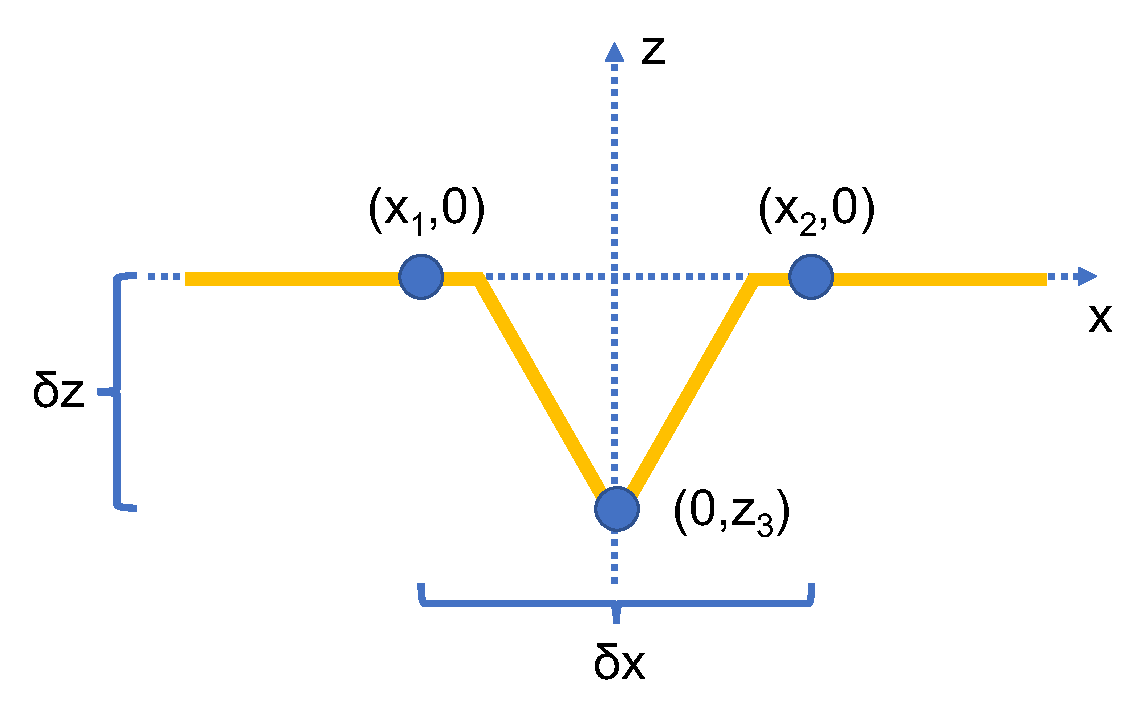
\includegraphics[width=.65\columnwidth]{model_three_sources.pdf} \vspace*{-0.25cm}
\caption{\label{fig:3source_layout}Simplified model of a surface crack with three point sources. We estimate the depth parameter $\delta z$ and width parameter $\delta x$.}
\end{figure}

This setup leads to the following QFIM structure
\begin{align}
    H &= \begin{pmatrix}
    \var{x_1} & \cov{x_1}{x_2} & \cdots & \cov{x_1}{z_3} \\
    \cov{x_2}{x_1} & \var{x_2} & \cdots & \cov{x_2}{z_3} \\
    \vdots & \vdots & \ddots & \vdots \\
    \cov{z_3}{x_1} & \cdots & \cdots & \var{z_3}
    \end{pmatrix},
\end{align}
which is a $9 \times 9$ matrix that we can collapse to a $2 \times 2$ matrix for estimating the parameters $\delta x, \delta z$ defined in Eq.~\eqref{eq:coordinate_jacobian} with the Jacobian matrix
\begin{align}
    B &= \begin{pmatrix}
    -\frac{1}{2} & \frac{1}{2} & 0 & \cdots & 0\\
    0 & \cdots & \cdots & 0 & -1
    \end{pmatrix}.
\end{align}

We can now compare the ultimate precision bounds to specific measurement schemes one might use to estimate these parameters. In particular, we will explore decomposing the image plane into a modal basis and compare it to the traditional intensity measurement estimation.


\subsection{\label{subsec:FI_ms_incoherent} Cramer-Rao bounds for incoherent point sources}
We will directly estimate the $\delta x, \delta z$ parameters in a general basis $\{ \phi_j \}$. Our object distribution in the case of three point sources is written as
\begin{align}
    F(r|\theta) = \frac{1}{3} \left \{ \delta \left [ x-\frac{\delta x}{2} \right ] + \delta \left [ x+\frac{\delta x}{2} \right ] + \delta \left [ -\delta z \right ] \right \}
\end{align}
with $\delta[x]$ the Dirac delta. Plugging it into Eq.~(\ref{eq:ms_prob}), we obtain the mode sorting probabilities
\begin{align}
    p_j(\delta x,\delta z) = \frac{1}{3} & \mbox{$\left \{ \abs{\braket{\phi_j}{\psi_1(x-\frac{\delta x}{2},y,0)} }^2 +
    \abs{\braket{\phi_j}{\psi_2(x+\frac{\delta x}{2},y,0)} }^2\right.$}   \nonumber \\
    & + \mbox{$ \left.  \abs{\braket{\phi_j}{\psi_3(x,y,-\delta z)} }^2 \right \}$}
\label{eq:prob_ms_3src}
\end{align}
for a particular mode $j$.

HERE FOR NOW TO TEST SOMETHING
\begin{align}
    J_{a,b} = \tau \sum_j\frac{1}{p_j(\theta)} \pdv{p_j(\theta)}{\theta_a}  \pdv{p_j(\theta)}{\theta_b}.
\label{eq:FI_MS}
\end{align}
WILL BE DELETED


Let us now assume that we can create a point-spread function adapted basis \cite{rehacek2017optimal} expressed as
\begin{align}
    \phi_j(x,y) &=\sum_\zeta^j c_\zeta x^\zeta \ \sqrt{\frac{1}{\pi}} \exp{\frac{-(x^2 + y^2)}{2}}\\
    &= \sum_\zeta^j c_\zeta x^\zeta \ \psi_0(x,y) \nonumber .
\end{align}
We then obtain the following closed-form expression for the measuring probabilities (see Appendix~\ref{app:ms_incoherent} for a complete derivation)
\begin{align}
    \abs{\braket{\phi_j}{\psi(x+\delta x,y,\delta z)}}^2 &= \frac{4}{4 + \delta z^2}\exp{-\frac{2\delta x^2}{4+\delta z^2}}\abs{\sum_\zeta^j c^*_\zeta \mathbb{E}[x^\zeta]}^2,
    \label{eq:three_sources_incoherent_ms_prob}
\end{align}
with $\mathbb{E}[x^\zeta]$ the moments of the Gaussian distribution that can be computed recursively via
\begin{align}
\label{def:recursive_moments}
    \mathbb{E}[x^{\zeta+1}] = \mu \mathbb{E}[x^\zeta] + \zeta \sigma^2 \mathbb{E}[x^{\zeta-1}]
\end{align}
and
\begin{align}
\label{def:mu_sigma}
&\mu = - \frac{i\delta x}{2i + \delta z}, \quad \frac{1}{2\sigma^2} = \frac{1}{2} \left[ 1 + \frac{i}{i + \delta z} \right], \\
&\mathbb{E}[x^0] = 1, \quad \mathbb{E}[x^1] = \mu.  \nonumber
\end{align}
This shows we can build the classical FIM by polynomial order Eq.~\eqref{eq:FI_MS} and analyze individual order contributions.

We demonstrate this analysis by using the first four Hermite polynomials \cite{weisstein2002hermite} with a point-spread function matching the Gaussian distribution
\begin{align}
    \phi_{j,0}(x,y) = \frac{H_j(x)}{\sqrt{2^j j!}} \sqrt{\frac{1}{\pi}} \exp{-\frac{(x^2 + y^2)}{2}}
\end{align}
with the first four moments
\begin{align}
    \mathbb{E}[x^0] &= 1 \\
    \mathbb{E}[x^1] &= -\frac{i \delta x}{2i + \delta z} \\
    \mathbb{E}[x^2] &= \frac{-2 + \delta z (3i + \delta z) - \delta x^2}{(2i + \delta z)^2} \\
    \mathbb{E}[x^3] &= \frac{\delta x (9 \delta z - 3i \delta z^2 + i (6 + \delta x^2))}{(2 i + \delta z)^3} \\
    \mathbb{E}[x^4] &= \frac{3 (-2 + 3 i \delta z + \delta z^2)^2 - 6 (i + \delta z) (2 i + \delta z) \delta x^2 + \delta x^4}{(2 i + \delta z)^4}
\end{align}
and the derivatives w.r.t. $\delta x,\delta z$ also lead to closed-form analytical solutions.

To make a comparison, we will benchmark against the classical intensity measurement in the image plane. In the incoherent regime, the intensities will add linearly, and we obtain the following distribution needed to calculate the classical Fisher information
\begin{align}
     P(x,y|\delta x,\delta z)=\! \mbox{$\dfrac{{|{\psi_1(x\!-\!\frac{\delta x}{2},y,0)}|^2\!\! + \!|{\psi_2(x\!+\!\frac{\delta x}{2},y,0)}|^2\!\! + \!|{\psi_3(x,y,-\delta z)}|^2}}{3}$}.
\end{align}


A closed-form solution cannot be derived analytically, and we use numerical integration to calculate the result.

\begin{figure*}
\centering
\subfloat[Estimation of the width parameter $\delta x$ for incoherent sources.]{\label{fig:incoh_MS_s}\includegraphics[width=\columnwidth]{three_sources_incoh_s.pdf}}\qquad
\subfloat[Estimation of the depth parameter $\delta z$ for incoherent sources.]{\label{fig:incoh_MS_p}\includegraphics[width=\columnwidth]{three_sources_incoh_p.pdf}}\\
\subfloat[Estimation of the width parameter $\delta x$ for coherent sources.]{\label{fig:coh_MS_s}\includegraphics[width=\columnwidth]{three_sources_coh_s.pdf}}\qquad
\subfloat[Estimation of the depth parameter $\delta z$ for coherent sources.]{\label{fig:coh_MS_p}\includegraphics[width=\columnwidth]{three_sources_coh_p.pdf}}%
\caption{Estimation of the parameters $\delta x$ [(a),(c)] and $\delta z$ [(b),(d)] as depicted in Fig.~\ref{fig:3source_layout}, for incoherent [(a),(b)] or coherent [(c),(d)] point sources. Contributions of individual Hermite-Gaussian modes, (0 - Red), (1 - Green), (2 - Purple), (3 - Orange), (4 - Gray), to the Fisher Information (Blue - MS), compared to the Quantum Fisher Information (Yellow-Pink - QFI) and the classical intensity measurement (Blue-Green).}
\label{4figs}
\end{figure*}


We can see that each parameter has a dominating contribution from a single Hermite polynomial. In the case of estimating the gap width, we can saturate the ultimate precision bound by measuring the first-order Hermite polynomial [Fig.~\ref{fig:incoh_MS_s}]. While we do not reach the precision boundary in the case of estimating the depth, we see the dominating contribution comes from the second-order Hermite polynomial [Fig.~\ref{fig:incoh_MS_s}]. In the small depth and gap regime, the Fisher information scales similar to the quantum Fisher information. In both cases, measuring more modes adds accuracy for a wider range of values but does not give a substantial contribution in the critical region. In the same critical region, we also see that measuring in the Hermite basis is beneficial as opposed to the classical intensity measurement.

\subsection{\label{subsec:FI_ms_coherent} Cramer-Rao bounds for coherent point sources}
For the sake of completeness we also evaluate the precision bounds in the case of coherent point sources. The same work calculating the coherent QFIM \cite{da2021super} also provides us with the expressions for calculating the FIM in the case of mode sorting

\begin{align}
    J^{MS}_{a,b} = 2 \Re \left \{ \sum_j \pdv{E^*_j}{\theta_a} \pdv{E_j}{\theta_b} \right \} + 2 \Re \left \{ \sum_j \pdv{E_j}{\theta_a} \pdv{E_j}{\theta_b} \frac{E^*_j}{E_j} \right \}.
\end{align}

Measuring Hermite polynomials of order $j$ in the image plane leads to the electric field distribution (particular case of the general expression derived in Appendix \ref{app:ms_incoherent})
%\begin{widetext}
\begin{align}
\label{eq:three_sources_coherent_ms_prob}
     E_j =\ & \frac{1}{3} \left [ \braket{\phi_j}{ \psi_1 (x+\mbox{$\frac{\delta x}{2}$},y,0)} + \braket{\phi_j}{\psi_2 (x-\mbox{$\frac{\delta x}{2}$},y,0)} \right. \nonumber \\
     &\left. + \braket{\phi_j}{\psi_3 (x,y,-\delta z)} \right ].
\end{align}


We can observe already from the electric field distribution that only modes with even parity will contribute to the estimation. For the classical intensity measurement we  will again have to resort to numerical integration as a closed-form solution cannot be found.



We see that estimating the gap width is already measurement optimal using the conventional intensity measurement [Fig.~\ref{fig:coh_MS_s}] and for narrow gaps it results in a bigger estimation error. Compared to the previous case however, we see that multiple even Hermite modes contribute roughly equally to the estimation accuracy, whereby odd modes do not contribute at all. In the case of estimating the depth neither Hermite modes nor the classical method are optimal and yield the same subpar result [Fig.~\ref{fig:coh_MS_p}]. This open the posibility of finding a better measurement for estimating this parameter. Surprisingly, for the Hermite modes only the zeroth order carries any substantial contribution, hence the overlap with the intensity measurement.

\section{\label{sec:conc} Conclusion}
This article presents a promising general approach for modelling surfaces via a discrete imaging model using point sources. By expanding the parameter space to estimate individual point source coordinates and then performing dimensionality reduction via coordinate transforms, we can derive descriptive parameters for surface characteristics. Our approach, which focuses on passive imaging schemes that allow single-shot profilometry, has the potential to significantly advance the field of optical surface metrology.
We demonstrate our technique on a simplified three-point source model that gives us an insight into practical measurements and can be used to represent surface defects. We find that incoherent light is better than coherent when estimating the width and gap of a surface crack. Furthermore, we find that in the case of incoherent light, each parameter of interest can be measured with improved accuracy using a modal measurement basis in the image plane. Our analysis also suggests that measurement basis vectors have a fuzzy one-to-one correspondence with descriptive parameters. In our case, it is possible to find two single point-spread function adapted basis polynomials, each respectively carrying the majority of information necessary to estimate the depth and width of the gap. This leads us to pose the question of whether such a correspondence can be shown in all generalty or if it has its limits.
More suitable measurements exist for estimating the depth in the case of coherent sources. This example showcases the difficulty in finding optimal measurements, as it can be a hit-or-miss situation. It would be beneficial to have a general approach in constructing measurement basis vectors that approach the ultimate precision bound.
Lastly, our work motivates two possible optimisation directions. Firstly, given a set of desired parameters to estimate, we can optimise the measurement basis to saturate the quantum Cramer-Rao bound. Secondly, we can explore parameters we can estimate with the ultimate precision for a given measurement basis set.


\begin{acknowledgments}
We thank some people.
\end{acknowledgments}

\clearpage
\appendix
\onecolumngrid
\section{\label{app:gaussian_overlaps}Closed form Gaussian overlaps for Grammian}
Matrix elements to show closed form expressions.
All overlaps share a common exponential factor
\begin{align}
    \psi_0 = \exp \left \{ (i \frac{(\delta_{x_v} - \delta_{x_u})^2 + (\delta_{y_v} - \delta_{y_u})^2)}{2(-2i + \delta_{z_v} - \delta_{z_u})} + i k z_R (\delta_{z_v} - \delta_{z_u}) \right \}
\end{align}

\begin{align}
    \braket{\psi_v}{\psi_u} &= \frac{2 i}{2 - \delta_{z_v} + \delta_{z_u}} \psi_0 \\
    \braket{\partial_{\delta_{x_v}}\psi_v}{\psi_u} &=  -2 \frac{\delta_{x_v} - \delta_{x_u}}{(2i - \delta_{z_v} + \delta_{z_u})^2} \psi_0\\
    \braket{\partial_{\delta_{y_v}}\psi_v}{\psi_u} &=  -2 \frac{\delta_{y_v} - \delta_{y_u}}{(2i - \delta_{z_v} + \delta_{z_u})^2} \psi_0\\
    \braket{\partial_{\delta_{z_v}}\psi_v}{\psi_u} &= \frac{-4 + (\delta_{x_v} - \delta_{x_u})^2 + (\delta_{y_v} - \delta_{y_u})^2 - 2 k z_R (-4 + (\delta_{z_v} - \delta_{z_u})^2) +  2i (\delta_{z_v} - \delta_{z_u})  (-1 + 4 k z_R)
    }{(-2i + \delta_{z_v} - \delta_{z_u})^3} \psi_0 \\
    \braket{\partial_{\delta_{x_v}}\psi_v}{\partial_{\delta_{x_u}}\psi_u} &= \frac{2i (-2 + (\delta_{x_v} - \delta_{x_u})^2 + i (\delta_{z_u} - \delta_{z_v}))}{(2i - \delta_{z_v} + \delta_{z_u})^3} \psi_0 \\
    \braket{\partial_{\delta_{x_v}}\psi_v}{\partial_{\delta_{y_u}}\psi_u} &= \frac{2i (\delta_{x_v} - \delta_{x_u}) (\delta_{y_v} - \delta_{y_u})}{ (2i - \delta_{z_v} + \delta_{z_u})^3} \psi_0 \\
    \braket{\partial_{\delta_{x_v}}\psi_v}{\partial_{\delta_{z_u}}\psi_u} &= -\frac{(-1 + i \delta_{z_u})^3 (\delta_{x_v} - \delta_{x_u}) \psi_0}{(i + \delta_{z_u})^3 (2i - \delta_{z_v} + \delta_{z_u})^4} \\
    &(-8 + (\delta_{x_v} - \delta_{x_u})^2 + (\delta_{y_v} - \delta_{y_u})^2  - 2 k z_R (-4 + (\delta_{z_v} - \delta_{z_u})^2) + 4i (\delta_{z_v} - \delta_{z_u}) (-1 + 2 k z_R)) \nonumber \\
    \braket{\partial_{\delta_{y_v}}\psi_v}{\partial_{\delta_{y_u}}\psi_u} &= 2i \frac{-2 + (\delta_{y_v} - \delta_{y_u})^2 + i (\delta_{z_u} - \delta_{z_v})}{ (2i - \delta_{z_v} + \delta_{z_u})^3} \psi_0\\
    \braket{\partial_{\delta_{y_v}}\psi_i}{\partial_{\delta_{z_u}}\psi_u} &= - \frac{(-1 + i \delta_{z_u})^3 (\delta_{y_v} - \delta_{y_u}) \psi_0}{(i + \delta_{z_u})^3 (2i - \delta_{z_v} + \delta_{z_u})^4}  \\
    & (-8 + (\delta_{x_v} - \delta_{x_u})^2 + (\delta_{y_v} - \delta_{y_u})^2 - 2 k z_R (-4 + (\delta_{z_v} - \delta_{z_u})^2) + 4i (\delta_{z_v} - \delta_{z_u}) (-1 + 2 k z_R)) \nonumber \\
    \braket{\partial_{\delta_{z_v}}\psi_v}{\partial_{\delta_{z_u}}\psi_u} &= \frac{i \psi_0}{2 (-2i + \delta_{z_v} - \delta_{z_u})^5} (  \\
    & -32 + 8 (\delta_{z_v} - \delta_{z_u})^2 - (\delta_{x_v} - \delta_{x_u})^2 ((\delta_{x_v} - \delta_{x_u})^2 + 2 (-8 + (\delta_{y_v} - \delta_{y_u})^2)) -(\delta_{y_v} - \delta_{y_u})^2 (-16 + (\delta_{y_v} - \delta_{y_u})^2) \nonumber \\
    &  + 64 k z_R + 4 k z_R
        (
            (\delta_{z_v} - \delta_{z_u})^2 (-12 + (\delta_{x_v} - \delta_{x_u})^2 + (\delta_{y_v} - \delta_{y_u})^2)
            - 4 ((\delta_{x_v} - \delta_{x_u})^2 + (\delta_{y_v} - \delta_{y_u})^2)
        ) \nonumber \\
    &- (2 k z_R)^2
        (
            (-4 + 4 \delta_{z_v} + \delta_{z_v}^2 - 2 (2 + \delta_{z_v}) \delta_{z_u} + \delta_{z_u}^2)
            (-4 + \delta_{z_v}^2 - 2 \delta_{z_v} (2 + \delta_{z_u}) + \delta_{z_u} (4 + \delta_{z_u}))
        ) \nonumber \\
    &+ i
        (8 (\delta_{z_v} - \delta_{z_u}) \nonumber \\
        &( -4 + (\delta_{x_v} - \delta_{x_u})^2 + (\delta_{y_v} - \delta_{y_u})^2 - k z_R (-12 + (\delta_{z_v} - \delta_{z_u})^2) \nonumber \\
        &- 2 k z_R ((\delta_{x_v} - \delta_{x_u})^2 + (\delta_{y_v} - \delta_{y_u})^2) + (2 k z_R)^2 (-4 + (\delta_{z_v} - \delta_{z_u})^2))))\nonumber
\end{align}


\section{\label{app:ms_incoherent}Derivation for measuring modes in the image plane}
We derive the closed-form overlap between a measurement mode and an arbitrarily displaced point source. We can then take the solution to express the measurement probabilities in Eqs.~\eqref{eq:three_sources_incoherent_ms_prob} and \eqref{eq:three_sources_coherent_ms_prob} for measuring in any point spread function adapted basis in the case of three point sources described by two parameters.

Without loss of generality, we can assume that the image plane is located at $z=0$, where the Gaussian beam has the most narrow waist, and the optical axis goes through the coordinate origin $x=y=0$. With this, the point source is displaced from the optical axis in the x-direction by $\delta_x$, in the y-direction by $\delta_y$, and displaced from the optimal z-position by $\delta_z$. We will express the measurement mode as general as $\phi_{j,l}(x,y) = g_j(x)f_l(y)\psi(x,y,0)$, where $g_j(x)$ (resp. $f_l(y)$) are polynomials of order $j$ (resp. $l$), but assume that the $x-y$ dimensions are separable. The measurement overlap between the point source distribution and our measuring mode becomes

\begin{align}
    \braket{\phi_{j,l}}{\psi(x+\delta_x,y+\delta_y,\delta_z)} &= \iint dxdy \  g^*_j(x) \ f^*_l(y) \ \psi(x,y,0) \ \psi(x+\delta_x,y,\delta_z) \nonumber \\
     &= \iint dxdy \ \left [  \sum_\zeta^j \sum_\xi^l c^*_\zeta d^*_\xi x^\zeta y^\xi \sqrt{\frac{1}{\pi}} \exp{-\frac{(x^2 + y^2)}{2}} \right ]^* \sqrt{\frac{1}{\pi}} \frac{i}{i + \delta_z}\exp{-i\frac{((x+\delta_x)^2 + y^2)}{2(i+\delta_z)} - i k z_R \delta_z} \nonumber \\
     &= \sum_\zeta^j  \sum_\xi^l c_\zeta^*  d_\xi^* \frac{1}{\pi} \frac{i \exp{-ikz_R \delta_z} \exp{\frac{i \delta_x^2}{2i+\delta_z}}}{i+\delta_z} \int dx \ x^\zeta \exp{-\frac{(x - \mu_x)^2}{2\sigma^2}} \int dy \ y^\xi \exp{-\frac{(y - \mu_y)^2}{2\sigma^2}},
\end{align}

with $\mu_x = i\delta_x / (2i + \delta_z), \mu_y = i\delta_y / (2i + \delta_z)$, and $\sigma$ having the same definition as in Eq.~\eqref{def:mu_sigma}. We can use the formula for complex-valued Gaussian integrals,

\begin{align}
    \int dx \ \exp{-ax^2} = \sqrt{\frac{\pi}{a}}
\end{align}

since $\Re{a} \geq 0$ will always hold. We can now express each integral as the generating functions of the moments for a normal distribution and obtain the result

\begin{align}
   \braket{\phi_{j,l}}{\psi(x+\delta_x,y+\delta_y,\delta_z)} &= \frac{2i}{2i + \delta_z}  \exp{-ikz_R\delta_z} \exp{-\frac{i}{2(2i +\delta_z)}(\delta_x^2 + \delta_y^2)} \sum_\zeta^j c^*_\zeta \mathbb{E}[x^\zeta]\sum_\xi^l d^*_\xi \mathbb{E}[y^\xi].
\end{align}

For the sake of completeness, we also derive the derivatives w.r.t. the point source displacements $(\delta_x,\delta_y,\delta_z)$ since we require them for calculating the classical Fisher information matrix of mode measurements. We begin with the derivatives of the electric field.

First, we centralize the random variable $x \sim \cal{N} (\mu,\sigma^2)$ by $x=\mu + \sigma Z$, where $Z \sim \cal{N} (0,1)$ and re-express the recurrence relation \eqref{def:recursive_moments} as a sum

\begin{align}
    \mathbb{E}[x^\zeta] = \mathbb{E}[(\mu + \sigma Z)^\zeta] = \sum_\alpha^\zeta \binom{\zeta}{\alpha} \mu^\alpha \sigma^{\zeta-\alpha} \mathbb{E}[Z^{\zeta-\alpha}],
\end{align}

where
\begin{align}
    \mathbb{E}[Z^{\zeta-\alpha}] = \begin{cases}
        \frac{(\zeta-\alpha)!}{2^{\frac{\zeta-\alpha}{2}} (\frac{\zeta-\alpha}{2})!} & \zeta-\alpha \text{ is even} \\
        0 & \text{else}
    \end{cases}.
\end{align}

It is easier now to derive a closed-form expression for the derivatives
\begin{align}
    \frac{\partial}{\partial \delta_x} \braket{\phi_{j,l}}{\psi(x+\delta_x,y+\delta_y,\delta_z)} &= \frac{2i}{2i + \delta_z}  \exp{-ikz_R\delta_z} \exp{-\frac{i \delta_y^2}{2(2i +\delta_z)}} \sum_\xi^l d^*_\xi \mathbb{E}[y^\xi]\sum_\zeta c^*_\zeta  \frac{\partial}{\partial \delta_x} \left [ \exp{-\frac{i\delta_x^2}{2(2i +\delta_z)}}\mathbb{E}[x^\zeta] \right ] \nonumber \\
    &=  \frac{2}{(2i + \delta_z)^2}  \exp{-ikz_R\delta_z} \exp{-\frac{i (\delta_x^2 + \delta_y^2)}{2(2i +\delta_z)}} \left ( \sum_\xi^l d^*_\xi \mathbb{E}[y^\xi] \right ) \left [ \delta_x \sum_\zeta c^*_\zeta \mathbb{E}[x^\zeta] \right. \nonumber \\
    & \left. + \sum_\zeta c^*_\zeta \sum^\zeta_\alpha \binom{\zeta}{\alpha} \alpha \mu_x^{\alpha-1} \sigma^{\zeta-\alpha}  \mathbb{E}[Z^{\zeta-\alpha}] \right ].
\end{align}

Similarly, by symmetry, we get the expression for the derivative in the y-dimension
\begin{align}
    \frac{\partial}{\partial \delta_y} \braket{\phi_{j,l}}{\psi(x+\delta_x,y+\delta_y,\delta_z)} &=  \frac{2}{(2i + \delta_z)^2}  \exp{-ikz_R\delta_z} \exp{-\frac{i (\delta_x^2 + \delta_y^2)}{2(2i +\delta_z)}} \left ( \sum_\zeta^j c^*_\zeta \mathbb{E}[x^\zeta] \right ) \left [ \delta_y \sum_\xi^l d^*_\xi \mathbb{E}[y^\xi] \right. \nonumber \\
    & \left. + \sum_\xi^l d^*_\xi \sum_\beta^\xi \binom{\xi}{\beta} \beta \mu_y^{\beta-1} \sigma^{\xi-\beta}  \mathbb{E}[Z^{\xi-\beta}] \right ].
\end{align}

Lastly, we have
\begin{align}
    \frac{\partial}{\partial \delta_z} &\braket{\phi_{j,l}}{\psi(x+\delta_x,y+\delta_y,\delta_z)} = \nonumber \\
    &\sum_\zeta^j c^*_\zeta \mathbb{E}[x^\zeta]\sum_\xi^l d^*_\xi \mathbb{E}[y^\xi] \frac{\partial}{\partial \delta_z} \left [ \frac{2i}{2i + \delta_z}  \exp{-ikz_R\delta_z} \exp{-\frac{i (\delta_x^2 + \delta_y^2)}{2(2i +\delta_z)}}  \right] \nonumber \\
    &+ \frac{2i}{2i + \delta_z}  \exp{-ikz_R\delta_z} \exp{-\frac{i (\delta_x^2 + \delta_y^2)}{2(2i +\delta_z)}} \frac{\partial}{\partial \delta_z} \left[ \sum_\zeta^j c^*_\zeta \mathbb{E}[x^\zeta]\sum_\xi^l d^*_\xi \mathbb{E}[y^\xi] \right] \nonumber \\
    &= \frac{2i}{2i + \delta_z}  \exp{-ikz_R\delta_z} \exp{-\frac{i (\delta_x^2 + \delta_y^2)}{2(2i +\delta_z)}} \Biggl [ \nonumber \\
    & \left(\frac{i(\delta_x^2 + \delta_y^2)}{2(2i + \delta_z)^2} - i k z_R - \frac{1}{2i + \delta_z} \right) \sum_\zeta^j c^*_\zeta \mathbb{E}[x^\zeta] \sum_\xi^l d^*_\xi \mathbb{E}[y^\xi] \nonumber \\
    & + \frac{1}{2i + \delta_zi} \sum_\xi^l d^*_\xi \mathbb{E}[y^\xi] \sum_\zeta^j c^*_\zeta \sum_\alpha^\zeta \binom{\zeta}{\alpha} \mathbb{E}[Z^{\zeta - \alpha}] \mu_x^\alpha \sigma^{\zeta-\alpha}\left ( \frac{\zeta-\alpha}{2} \frac{1}{\sigma^2} - \frac{\zeta + \alpha}{2} \right ) \nonumber \\
    & + \frac{1}{2i + \delta_z} \sum_\zeta^j c^*_\zeta \mathbb{E}[x^\zeta] \sum_\xi^l d^*_\xi \sum_\beta^\xi \binom{\xi}{\beta} \mathbb{E}[Z^{\xi - \beta}] \mu_y^\beta \sigma^{\xi-\beta}\left ( \frac{\xi-\beta}{2} \frac{1}{\sigma^2} - \frac{\xi + \beta}{2} \right ) \nonumber \\
    & \Biggr ]
\end{align}

\twocolumngrid
\nocite{*}
\bibliography{ref}% Produces the bibliography via BibTeX.

\end{document}
%
% ****** End of file apssamp.tex ******


\begin{figure}
\includegraphics[width=\columnwidth]{three_sources_inverse_coh_s.pdf}
\caption{\label{fig:inv_coh_MS_s} Estimation of the parameter $s$ for coherent point sources. Contributions of individual HG modes for coherent point sources, (0 - Red), (1 - Green), (2 - Purple), (3 - Orange), (4 - Gray), for the classical Fisher Information (Blue- MS) compared to the Quantum Fisher Information (Yellow-Pink - QFI) and the classical intensity measurement (Blue-Green).}
\end{figure}

\begin{figure}
\includegraphics[width=\columnwidth]{three_sources_inverse_coh_p.pdf}
\caption{\label{fig:inv_coh_MS_p} Estimation of the parameter $p$ for coherent point sources. Contributions of individual HG modes for coherent point sources, (0 - Red), (1 - Green), (2 - Purple), (3 - Orange), (4 - Gray), for the classical Fisher Information (Blue- MS) compared to the Quantum Fisher Information (Yellow-Pink - QFI) and the classical intensity measurement (Blue-Green).}
\end{figure}

\begin{figure}
\includegraphics[width=\columnwidth]{three_sources_inverse_incoh_s.pdf}
\caption{\label{fig:inv_incoh_MS_s} Estimation of the parameter $s$ for incoherent point sources. Contributions of individual HG modes for incoherent point sources, (0 - Red), (1 - Green), (2 - Purple), (3 - Orange), (4 - Gray), for the classical Fisher Information (Blue- MS) compared to the Quantum Fisher Information (Yellow-Pink - QFI) and the classical intensity measurement (Blue-Green).}
\end{figure}

\begin{figure}
\includegraphics[width=\columnwidth]{three_sources_inverse_incoh_p.pdf}
\caption{\label{fig:inv_incoh_MS_p} Estimation of the parameter $p$ for incoherent point sources. Contributions of individual HG modes for incoherent point sources, (0 - Red), (1 - Green), (2 - Purple), (3 - Orange), (4 - Gray), for the classical Fisher Information (Blue- MS) compared to the Quantum Fisher Information (Yellow-Pink - QFI) and the classical intensity measurement (Blue-Green).}
\end{figure}
